
\documentclass{beamer}
\usecolortheme{dove}
\setbeamertemplate{navigation symbols}{}
\usepackage{amsmath,amssymb,amsfonts,amsthm, multicol, subfigure, color}
\usepackage{bm}
\usepackage{graphicx}
\usepackage{tabularx}
\usepackage{booktabs}
\usepackage{hyperref}
\usepackage{pdfpages}
\usepackage{xcolor}
\definecolor{seagreen}{RGB}{46, 139, 87}
\definecolor{mustard}{RGB}{234, 170, 0}
\def\independenT#1#2{\mathrel{\rlap{$#1#2$}\mkern2mu{#1#2}}}
\newcommand\indep{\protect\mathpalette{\protect\independenT}{\perp}}
\def\log{\text{log}}
\newcommand\logit{\text{logit}}
\newcommand\iid{\stackrel{\text{iid}}{\sim}}
\newcommand\E{\text{E}}
\newcommand\V{\text{V}}
\renewcommand\P{\text{P}}
\newcommand{\Cov}{\text{Cov}}
\newcommand{\Cor}{\text{Cor}}
\newcommand\doop{\texttt{do}}
\usepackage{stackrel}
\usepackage{tikz}
\usetikzlibrary{arrows,shapes.arrows,positioning,shapes,patterns,calc}
\newcommand\slideref[1]{\vskip .1cm \tiny \textcolor{gray}{{#1}}}
\newcommand\red[1]{\color{red}#1}
\newcommand\blue[1]{\color{blue}#1}
\newcommand\gray[1]{\color{gray}#1}
\newcommand\seagreen[1]{\color{seagreen}#1}
\newcommand\purple[1]{\color{purple}#1}
\newcommand\orange[1]{\color{orange}#1}
\newcommand\black[1]{\color{black}#1}
\newcommand\white[1]{\color{white}#1}
\newcommand\teal[1]{\color{teal}#1}
\newcommand\magenta[1]{\color{magenta}#1}
\newcommand\Fuchsia[1]{\color{Fuchsia}#1}
\newcommand\BlueGreen[1]{\color{BlueGreen}#1}
\newcommand\bblue[1]{\textcolor{blue}{\textbf{#1}}}
\newcommand\bred[1]{\textcolor{red}{\textbf{#1}}}
\newcommand\bgray[1]{\textcolor{gray}{\textbf{#1}}}
\newcommand\bgreen[1]{\textcolor{seagreen}{\textbf{#1}}}
\newcommand\bref[2]{\href{#1}{\color{blue}{#2}}}
\colorlet{lightgray}{gray!40}
\pgfdeclarelayer{bg}    % declare background layer for tikz
\pgfsetlayers{bg,main} % order layers for tikz
\newcommand\mycite[1]{\begin{scriptsize}\textcolor{darkgray}{(#1)}\end{scriptsize}}
\newcommand{\tcframe}{\frame{
%\small{
\only<1|handout:0>{\tableofcontents}
\only<2|handout:1>{\tableofcontents[currentsubsection]}}
%}
}

\newcommand{\goalsframe}{\begin{frame}{Learning goals for today}
By the end of class, you will be able to
\begin{itemize}
    \item connect causal inference\hfill (a missing data problem)\vskip .1in to statistical modeling\hfill (predicting missing data)
\end{itemize} \vskip .2in
\end{frame}}

\usepackage[round]{natbib}
\bibliographystyle{humannat-mod}
\setbeamertemplate{enumerate items}[default]
\usepackage{mathtools}

\title{Studying Social Inequality with Data Science}
\author{Ian Lundberg}
\date{\today}

\begin{document}

\begin{frame}
\begin{tikzpicture}[x = \textwidth, y = \textheight]
\node at (0,0) {};
\node at (1,1) {};
\node[anchor = north west, align = left, font = \huge] at (0,.9) {Social\\Data\\Science};
\node[anchor = north east, align = right] (number) at (1,.9) {SOCIOL 114\\Winter 2025};
\node[anchor = north, font = \Large, align = left] at (.5,.5) {\bblue{Causal inference:}\\\bblue{Connections to statistical modeling}};
\end{tikzpicture}
\end{frame}

\goalsframe

\begin{frame}{A running example}

I feel confident that I can answer quantitative questions with tools from data science. \vskip .1in

\begin{itemize}
\item 1 = Agree
\item 0 = Disagree
\end{itemize} \vskip .3in \pause
What is the average causal effect of taking this class\\
on confidence in data science skills?

\end{frame}

\begin{frame}{Using potential outcomes}


\begin{tikzpicture}[x = \textwidth, y = .8\textheight]
\node at (0,0) {};
\node at (1,1) {};
\foreach \i in {.3, .4, .5,.6,.7,.8} {
	\draw[fill = blue, opacity = .3, color = blue] (.05,\i) rectangle (.25,\i + .1) {};
	\draw[fill = seagreen, opacity = .3, color = seagreen] (.25,\i) rectangle (.45,\i + .1) {};
}
\node[font = \footnotesize] at (.15,.85) {$Y_1^\text{Takes 114}$};
\node[font = \footnotesize] at (.15,.75) {$Y_2^\text{Takes 114}$};
\node[font = \footnotesize] at (.15,.55) {$Y_4^\text{Takes 114}$};
\node[font = \footnotesize] at (.15,.65) {$Y_3^\text{Takes 114}$};
\node[font = \footnotesize] at (.15,.45) {$Y_5^\text{Takes 114}$};
\node[font = \footnotesize] at (.15,.35) {$Y_6^\text{Takes 114}$};
\only<1>{
\node[font = \footnotesize] at (.35,.85) {$Y_1^\text{No 114}$};
\node[font = \footnotesize] at (.35,.75) {$Y_2^\text{No 114}$};
\node[font = \footnotesize] at (.35,.55) {$Y_4^\text{No 114}$};
\node[font = \footnotesize] at (.35,.65) {$Y_3^\text{No 114}$};
\node[font = \footnotesize] at (.35,.45) {$Y_5^\text{No 114}$};
\node[font = \footnotesize] at (.35,.35) {$Y_6^\text{No 114}$};
}
\only<2->{
\node[font = \footnotesize] at (.35,.85) {?};
\node[font = \footnotesize] at (.35,.75) {?};
\node[font = \footnotesize] at (.35,.55) {?};
\node[font = \footnotesize] at (.35,.65) {?};
\node[font = \footnotesize] at (.35,.45) {?};
\node[font = \footnotesize] at (.35,.35) {?};
}
\node[anchor = north, align = center, font = \footnotesize, blue] at (.15, .3) {Outcome\\under\\114};
\node[anchor = north, align = center, font = \footnotesize, seagreen] at (.35, .3) {Outcome\\under\\no 114};
\node[anchor = south, rotate = 90, align = center] at (.05, .6) {Each Row is a\\Student in This Class};
\node[anchor = north west, align = left, font = \footnotesize, align = left] at (.55,1) {$Y$ = I feel confident that I can\\answer quantitative questions\\with tools from data science};
\node<3->[anchor = north west, align = left, align = left] at (.55,.6) {How could we learn\\about the (?)};
\end{tikzpicture}

\end{frame}

\begin{frame}{Strategy 1: A subgroup with conditional exchangeability} \pause

\begin{itemize}
\item Some of the class was on the waitlist
\begin{itemize}
\item some got in
\item others didn't
\end{itemize}
\end{itemize}

\end{frame}

\begin{frame}{Strategy 1: A subgroup with conditional exchangeability}


\begin{tikzpicture}[x = \textwidth, y = .8\textheight]
\node at (0,0) {};
\node at (1,1) {};
\foreach \i in {.1,.2,.3, .4, .5,.6,.7,.8} {
	\draw[fill = blue, opacity = .3, color = blue] (.05,\i) rectangle (.25,\i + .1) {};
	\draw[fill = seagreen, opacity = .3, color = seagreen] (.25,\i) rectangle (.45,\i + .1) {};
}
\node[font = \footnotesize] at (.15,.85) {$Y_1^\text{Takes 114}$};
\node[font = \footnotesize] at (.15,.75) {$Y_2^\text{Takes 114}$};
\node[font = \footnotesize] at (.15,.65) {$Y_3^\text{Takes 114}$};
\node[font = \footnotesize] at (.15,.55) {$Y_4^\text{Takes 114}$};
\node[font = \footnotesize] at (.15,.45) {?};
\node[font = \footnotesize] at (.15,.35) {?};
\node[font = \footnotesize] at (.15,.25) {?};
\node[font = \footnotesize] at (.15,.15) {?};
\node[font = \footnotesize] at (.35,.85) {?};
\node[font = \footnotesize] at (.35,.75) {?};
\node[font = \footnotesize] at (.35,.65) {?};
\node[font = \footnotesize] at (.35,.55) {?};
\node[font = \footnotesize] at (.35,.45) {$Y_5^\text{No 114}$};
\node[font = \footnotesize] at (.35,.35) {$Y_6^\text{No 114}$};
\node[font = \footnotesize] at (.35,.25) {$Y_7^\text{No 114}$};
\node[font = \footnotesize] at (.35,.15) {$Y_8^\text{No 114}$};
\draw<2->[fill = gray] (.47,.71) rectangle (.57,.89);
\node<2->[white, font = {\bf\scriptsize}, align = center] at (.52,.8) {Pre-\\Enroll};
\draw<2->[fill = gray] (.47,.31) rectangle (.57,.69);
\node<2->[white, font = {\bf\scriptsize}, align = center] at (.52,.5) {Waitlist};
\draw<2->[fill = gray] (.47,.11) rectangle (.57,.29);
\node<2->[white, font = {\bf\scriptsize}, align = center] at (.52,.2) {No\\Interest};
%\node[anchor = north, align = center, font = \footnotesize, blue] at (.15, .3) {Outcome\\under\\114};
%\node[anchor = north, align = center, font = \footnotesize, seagreen] at (.35, .3) {Outcome\\under\\no 114};
\node[anchor = south, rotate = 90, align = center] at (.05, .45) {Each Row is a\\Student in This Class};
\node[anchor = north west, align = left, font = \footnotesize, align = left] at (.55,1) {$Y$ = I feel confident that I can\\answer quantitative questions\\with tools from data science};
\onslide<3->{
\draw[color = white, fill = white, fill opacity = .8] (.05,.1) rectangle (.6,.3);
\draw[color = white, fill = white, fill opacity = .8] (.05,.7) rectangle (.6,.9);
}
\node<4->[anchor = north west, align = left, font = \bf] (benefits) at (.6,.7) {Benefits of strategy};
\node<4->[anchor = north west, align = left, font = \bf] (drawbacks) at (.6,.5) {Drawbacks};
\node<5->[anchor = north west] at (benefits.south west) {Credible};
\node<5->[anchor = north west] at (drawbacks.south west) {Limited target population};
\end{tikzpicture}

\end{frame}

\begin{frame}{Strategy 2: Adjust for measured confounders} \pause

For each of you, we could compare
\begin{enumerate}
\item your opinion after 114
\item the average opinion of non-114 students who look like you
\end{enumerate} \pause
\vskip .3in
Looks like you in what ways? What else belongs in this DAG? \vskip .2in
\begin{center}

\begin{tikzpicture}[x = 2.5in, y = .5in]
\node[align = center] (a) at (0,0) {Takes a class\\``Social Data Science''};
\node[align = center] (y) at (1,0) {Confident in\\data science skills};
\draw[->, thick] (a) -- (y);
\end{tikzpicture}
\end{center}

\end{frame}

\begin{frame}{Strategy 2: Adjust for measured confounders}

\begin{center}
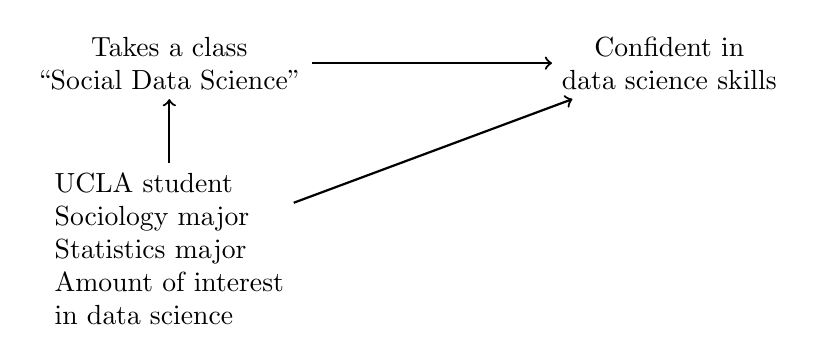
\begin{tikzpicture}[x = 2.5in, y = .5in]
\node[align = center] (a) at (0,0) {Takes a class\\``Social Data Science''};
\node[align = center] (y) at (1,0) {Confident in\\data science skills};
\draw[->, thick] (a) -- (y);
\node[anchor = north, align = left] (x) at (0,-1) {UCLA student\\Sociology major\\Statistics major\\Amount of interest\\in data science};
\draw[->, thick] (x) -- (a);
\draw[->, thick] (x) -- (y);
\end{tikzpicture}
\end{center}
Suppose these are a sufficient adjustment set.

\end{frame}

\begin{frame}{Strategy 2: Adjust for measured confounders}

\textbf{Nonparametric estimation:}\vskip .1in
For each student in the class, find someone else who
\begin{itemize}
\item is a student at UCLA
\item shares your major
\item is exactly as interested in data science as you are
\item but did not take this class
\end{itemize} \vskip .1in
Use your \textbf{match} to infer your $Y_i^\text{No 114}$ for people like you:

$$\E(Y^0\mid \vec{X} = \vec{x}_i) = \underbrace{\E(Y\mid A = 0,\vec{X} = \vec{x}_i)}_\text{estimated from your match}$$
since we have assumed conditional exchangeability given $\vec{X}$.

\end{frame}

\begin{frame}{Generalizing to a model}

\begin{tikzpicture}[x = \textwidth, y = .9\textheight]
\node[anchor = west] at (.75,.5) {\includegraphics{figures/legend}};
\node<1>[anchor = west] at (0,.5) {\includegraphics{figures/p1}};
\node<2>[anchor = west] at (0,.5) {\includegraphics{figures/p2}};
\node<3>[anchor = west] at (0,.5) {\includegraphics{figures/p3}};
\node<4>[anchor = west] at (0,.5) {\includegraphics{figures/p4}};
\node<5>[anchor = west] at (0,.5) {\includegraphics{figures/p5}};
\node<1>[anchor = west] at (0,.1) {1) Find control units who didn't take this class};
\node<2>[anchor = west] at (0,.1) {2) Model their outcomes given pre-treatment variables};
\node<3>[anchor = west] at (0,.1) {3) Find the treated units of interest};
\node<4>[anchor = west] at (0,.1) {4) Predict their counterfactual outcomes};
\node<5>[anchor = west] at (0,.1) {5) Infer causal effect for each person. Average over people};
\end{tikzpicture}

\end{frame}

\begin{frame}{Strategy 2: Generalizing to a model}

\begin{tikzpicture}[x = \textwidth, y = .9\textheight]
%\node[anchor = west] at (.75,.9) {\includegraphics{legend}};
\node[anchor = west] at (.75,.9) {\includegraphics[scale = .3]{figures/p1}};
\node[anchor = west] at (.75,.7) {\includegraphics[scale = .3]{figures/p2}};
\node[anchor = west] at (.75,.5) {\includegraphics[scale = .3]{figures/p3}};
\node[anchor = west] at (.75,.3) {\includegraphics[scale = .3]{figures/p4}};
\node[anchor = west] at (.75,.1) {\includegraphics[scale = .3]{figures/p5}};
\node[anchor = west, scale = .8] at (0,.9) {1) Find control units who didn't take this class};
\node[anchor = west, scale = .8] at (0,.7) {2) Model their outcomes given pre-treatment variables};
\node[anchor = west, scale = .8] at (0,.5) {3) Find the treated units of interest};
\node[anchor = west, scale = .8] at (0,.3) {4) Predict their counterfactual outcomes};
\node[anchor = west, scale = .8] at (0,.1) {5) Infer causal effect for each person. Average over people};
\end{tikzpicture}

\end{frame}

\begin{frame}{Summary: Outcome model for causal inference}


\begin{tikzpicture}[x = \textwidth, y = .8\textheight]
\node at (0,0) {};
\node at (1,1) {};
\foreach \i in {.3, .4, .5,.6,.7,.8} {
	\draw[fill = blue, opacity = .3, color = blue] (.05,\i) rectangle (.25,\i + .1) {};
	\draw[fill = seagreen, opacity = .3, color = seagreen] (.25,\i) rectangle (.45,\i + .1) {};
}
\node[font = \footnotesize] at (.15,.85) {$Y_1^\text{Takes 114}$};
\node[font = \footnotesize] at (.15,.75) {$Y_2^\text{Takes 114}$};
\node[font = \footnotesize] at (.15,.55) {$Y_4^\text{Takes 114}$};
\node[font = \footnotesize] at (.15,.65) {$Y_3^\text{Takes 114}$};
\node[font = \footnotesize] at (.15,.45) {$Y_5^\text{Takes 114}$};
\node[font = \footnotesize] at (.15,.35) {$Y_6^\text{Takes 114}$};
\only<1>{
\node[font = \footnotesize] at (.35,.85) {?};
\node[font = \footnotesize] at (.35,.75) {?};
\node[font = \footnotesize] at (.35,.55) {?};
\node[font = \footnotesize] at (.35,.65) {?};
\node[font = \footnotesize] at (.35,.45) {?};
\node[font = \footnotesize] at (.35,.35) {?};
}
\only<2->{
\node[font = \footnotesize] at (.35,.85) {$\hat{Y}_1^\text{No 114}$};
\node[font = \footnotesize] at (.35,.75) {$\hat{Y}_2^\text{No 114}$};
\node[font = \footnotesize] at (.35,.55) {$\hat{Y}_4^\text{No 114}$};
\node[font = \footnotesize] at (.35,.65) {$\hat{Y}_3^\text{No 114}$};
\node[font = \footnotesize] at (.35,.45) {$\hat{Y}_5^\text{No 114}$};
\node[font = \footnotesize] at (.35,.35) {$\hat{Y}_6^\text{No 114}$};
}
\node[anchor = north, align = center, font = \footnotesize, blue] at (.15, .3) {Outcome\\under\\114};
\node[anchor = north, align = center, font = \footnotesize, seagreen] at (.35, .3) {Outcome\\under\\no 114};
\node[anchor = south, rotate = 90, align = center] at (.05, .6) {Each Row is a\\Student in This Class};
\node<3->[anchor = north west] at (.52,.9) {\textbf{General approach}};
\node<4->[anchor = north west] at (.52,.8) {1) Define potential outcomes};
\node<5->[anchor = north west] at (.52,.72) {2) Define target population};
\node<6->[anchor = north west] at (.52,.64) {3) Make causal assumptions};
\node<7->[anchor = north west] at (.52,.56) {4) Model unobserved outcomes};
\node<8->[anchor = north west] at (.52,.48) {5) Predict them};
\node<9->[anchor = north west] at (.52,.4) {6) Report an average};
\end{tikzpicture}

\end{frame}

\goalsframe

\end{document}





